%!TEX options=--shell-escape
\documentclass[tikz]{standalone}
\usepackage[T1]{fontenc}
\usepackage[utf8]{inputenc}
\usepackage{xcolor}
\usepackage{amsmath}
\usepackage{amssymb}
\usepackage{hyperref}
\usepackage{accsupp}    
\usepackage{graphicx}
\usepackage{mathtools}
\usepackage{pagecolor}
\usepackage{amsmath} % for \dfrac
\usepackage{tikz,ifthen}
\tikzset{>=latex} % for LaTeX arrow head
\usepackage{braket}
\usepackage{pgfplots} 
\usepackage[edges]{forest}
\usetikzlibrary{patterns, backgrounds, arrows.meta}
\setlength{\parindent}{0cm}
\setlength{\parskip}{1em}

\usetikzlibrary{patterns, calc, intersections}

\def\rescale{0.1}
\def\innerwidth{25}
\def\outerwidth{53}
\def\innerlength{35}
\def\trackwidthmax{15}
\def\trackwidthmin{13}
\def\trackarcoffset{1}

\def\pageoffset{5}

\def\pagetop{\trackwidthmax  + 0.5 * \innerwidth + \pageoffset}
\def\pageleft{\trackwidthmax  + 0.5 * \innerwidth + \pageoffset}
\def\pageright{\trackwidthmax  + 0.5 * \innerwidth + \pageoffset}


\begin{document}
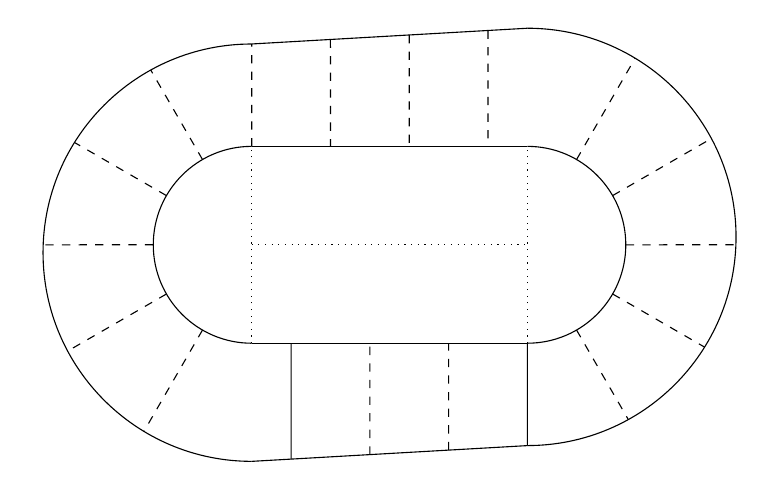
\begin{tikzpicture}[scale=\rescale]


%\draw(-2.5, \pagebottom) rectangle (5, \pagetop);

% Inside Rectangle

% TODO Coordinate this
\coordinate[](center) at (0,  0) {};
\coordinate[](center_left) at (-0.5 * \innerlength,  0) {};
\coordinate[](center_right) at (0.5 * \innerlength,  0) {};

\coordinate[](track_inner_right_bottom) at ([yshift=-0.5* \innerwidth cm]center_right) {};
\coordinate[](track_inner_right_top) at ([yshift=0.5*\innerwidth cm]center_right) {};

\coordinate[](track_inner_left_bottom) at ([yshift=-0.5* \innerwidth cm]center_left) {};
\coordinate[](track_inner_left_top) at ([yshift=0.5*\innerwidth cm]center_left) {};

\coordinate[](track_inner_left_offset) at ([yshift=-\trackarcoffset cm]center_left) {};
\coordinate[](track_inner_right_offset) at ([yshift=+\trackarcoffset cm]center_right) {};

\coordinate[](track_outer_left_bottom) at ([yshift=-0.5* \outerwidth cm]track_inner_left_offset) {};
\coordinate[](track_outer_left_top) at ([yshift=0.5*\outerwidth cm]track_inner_left_offset) {};

\coordinate[](track_outer_right_bottom) at ([yshift=-0.5* \outerwidth cm]track_inner_right_offset) {};
\coordinate[](track_outer_right_top) at ([yshift=0.5 * \outerwidth cm]track_inner_right_offset) {};


\coordinate[](track_outer_left) at ([xshift=-0.5 * \outerwidth cm]track_inner_left_offset) {};
\coordinate[](track_outer_right) at ([xshift=0.5 * \outerwidth cm]track_inner_right_offset) {};




\draw[dotted] (center_left) -- (center_right);
\draw[dotted] (track_inner_right_bottom) -- (track_inner_right_top);
\draw[dotted] (track_inner_left_bottom) -- (track_inner_left_top);
%
%\draw[dotted] (track_outer_left) -- (track_inner_left_offset);
%\draw[dotted] (track_outer_right) -- (track_inner_right_offset);


\draw[] (track_inner_left_bottom) -- (track_inner_right_bottom);
\draw[] (track_inner_left_top) -- (track_inner_right_top);
\draw[name path=track_outer_bottom] (track_outer_left_bottom) -- (track_outer_right_bottom);
\draw[name path=track_outer_top] (track_outer_left_top) -- (track_outer_right_top);


\draw[name path=apex_left_inner] (track_inner_left_bottom) arc (270:90:0.5 * \innerwidth);
\draw[name path=apex_right_inner] (track_inner_right_top) arc (270:90:-0.5 * \innerwidth);

\draw[name path=apex_left_outer] (track_outer_left_bottom) arc (270:90:0.5 * \outerwidth);
\draw[name path=apex_right_outer] (track_outer_right_top) arc (270:90:-0.5 * \outerwidth);

\draw[] (track_inner_right_bottom) -- (track_outer_right_bottom);
\draw[dashed] (track_inner_left_top) -- (track_outer_left_top);

\foreach \i in {1, 2, 3}{
    \coordinate[](ft_marker_bottom_center) at ([xshift = -10 * \i cm]track_inner_right_bottom);
    \coordinate[](ft_marker_bottom_outer) at ([yshift=-0.52 * \outerwidth cm + 0.5 * \innerwidth cm]ft_marker_bottom_center);
    \path[name path=ft_marker_bottom](ft_marker_bottom_outer) -- (ft_marker_bottom_center);  
    \path[name intersections={of=ft_marker_bottom and track_outer_bottom,by=ft_outer_bottom}];
    \ifthenelse{\i < 3}{
        \draw[dashed] (ft_outer_bottom) -- (ft_marker_bottom_center); 
    }{
        \draw[] (ft_outer_bottom) -- (ft_marker_bottom_center); 
    }
}  

\foreach \i in {1, 2, 3}{
    \coordinate[](ft_marker_top_center) at ([xshift= 10 * \i cm]track_inner_left_top);
    \coordinate[](ft_marker_top_outer) at ([yshift=0.52 * \outerwidth cm - 0.5 * \innerwidth cm]ft_marker_top_center);
    \path[name path=ft_marker_top](ft_marker_top_outer) -- (ft_marker_top_center);  
    \path[name intersections={of=ft_marker_top and track_outer_top,by=ft_outer_top}];
    \draw[dashed] (ft_outer_top) -- (ft_marker_top_center); 
}





\foreach \i in {1, 2, 3, 4, 5}{
    \path[name path=apex_marker](center_right) --++ (xy polar cs:angle=-90 + 30 * \i,radius=1cm);
    \path[name intersections={of=apex_marker and apex_right_inner,by=apex_inner}];
    \path[name intersections={of=apex_marker and apex_right_outer,by=apex_outer}];
    \draw[dashed] (apex_inner) -- (apex_outer);

    \path[name path=apex_marker](center_left) --++ (xy polar cs:angle=90 + 30 * \i,radius=1cm);
    \path[name intersections={of=apex_marker and apex_left_inner,by=apex_inner}];
    \path[name intersections={of=apex_marker and apex_left_outer,by=apex_outer}];
    \draw[dashed] (apex_inner) -- (apex_outer);
}

\end{tikzpicture} 
\end{document}

